

\section{Test Coverage Metrics}
\label{sec:coverage}
%Traditional test coverage metrics
%% over regular expressions fall short. 
%%Statement coverage just requires that the regular expression be executed. 
%%If the regular expression appears at a branching statement, branch coverage requires that the regular expression be tested with a matching string and a non-matching string~\cite{ammann2016introduction}.
%%However, these metrics 
%ignore much of the complexity within the regular expression. 
We explore fine-grained coverage metrics for regular expressions based on a DFA representation. 
The intuition is that since regular expressions are equivalent to DFAs~\cite{sipser2006introduction}, and 96\% of regular expressions in the wild were found to be regular (Section~\ref{regularregularexpressions}), then graph coverage metrics over the DFA can be used to test the behavior within the regular expression.  
We discuss three levels of coverage: Node Coverage (NC), Edge Coverage (EC), and Edge-Pair Coverage (EPC). These coverage metrics are adopted from graph coverage metrics proposed by Ammann and Offutt~\cite[Chapter 7]{ammann2016introduction}. 
%We explore these coverage metrics in the context of real programs in Section~\ref{sec:rq2}. 
%, and Exit Coverage (EXC)
%\todo{Adopt standard graph notation here, derived from the text, recognizing the text as the source. In standard graph notation, $G = \{V, E\}$. In our work, as in the text, we have special groups of nodes since we are working with DFAs. A graph $G = \{N, N_0, N_f, E\}$ where: $N$ is the set of all nodes, $N_0$ is a set of initial nodes, $N_f$ is a set of final nodes (in our case of DFAs, these are accept nodes), and $E$ is a set of edges}.

%\todo{check whole paper to make sure it's clear that $N_m$ is a set of matching nodes, and if the processing terminates at some $n \in N_m$, then the string is accepted.}
\subsection{Graph Notation} 
For ease of exposition, we expand on the traditional definition of a DFA. In this work, a DFA graph $G = \{N, N_0, N_m, N_e, E\}$ where: $N$ is the set of all nodes, $N_0$ is the initial node, $N_m$ is the final matching/accept node, $N_e$ is the final failing/error node, and $E$ is a set of all edges. 
%\todo{do we need a function to label the edges, like $B(e) = 0-9$ where $e = \overrightarrow{01}$?}
For the DFAs in this work, there is only one initial state, one accept state, and one error state.\footnote{In a FullMatch DFA (see Section~\ref{rq1instrumentation}), there could be several matching nodes, and only one accept. We simplified to use only one accept state.}

The states in a DFA are the nodes $N = \{n_0, n_1, \dots, n_k\}$. 
For any two nodes $n_1$ and $n_2$ such that $\{n_1, n_2\} \subseteq N$, if there is a transition from $n_1$ to $n_2$ in DFA, then the edge $\overrightarrow{n_1n_2} \in E$;  the start and end-state of the path may be the same node, as is the case of self-loops. 
Edge pairs are defined by paths of length two in the DFA.
For example,  if \{$\overrightarrow{n_1n_2}, \overrightarrow{n_2n_3}\} \in E$,  we denote the edge pair as $\overrightarrow{n_1n_2n_3}$.
In the case of self-loops, $\overrightarrow{n_2n_2n_2}$ is also a valid edge-pair. % \in EP$ or $\overrightarrow{n_1n_3n_4} \in EP$. 

Given an input string and a regular expression, the initial node $N_0$ is visited first. Transitions are taken as each character in the string is consumed. The result of the matching process ends in either the accept node $N_m$ or the error node $N_e$. 
In standard DFAs, a traversal can end in any node. However, the DFA generation algorithm used in this work is based on the RE2 tool, which always ends processing in an explicit matching/accept ($N_m$) or error ($N_e$) state.
In this tool, given a regular expression and an input string, the input string is interpreted as a byte stream, with byte {\tt [256]} added to the end to mark the end of the string. Thus, an input string ``2'' would be interpreted as {\tt [50 256]} and the input string ``1001'' would be interpreted as {\tt [49 48 48 49 256]}. 

\looseness +1
As a running example, consider regular expression  $R$ = \verb!\d+! and graph $G$  in Figure ~\ref{fig:static}. %This is a forward-processing DFA, that is, processing of the string starts at the front of the regular e
In $G$, $N~=~\{0, 1, 2, 3, E\}$, $N_0 = 0$, $N_m = 3$, $N_e = e$, 
$E~=~\{\overrightarrow{0e}, \overrightarrow{01}, \overrightarrow{12}, \overrightarrow{13}, \overrightarrow{22}, \overrightarrow{23}, \overrightarrow{3e}\}$, and\\ 
$EP~=~\{\overrightarrow{012}, \overrightarrow{013}, \overrightarrow{122}, \overrightarrow{123},
\overrightarrow{13e}, \overrightarrow{222}, \overrightarrow{223}, \overrightarrow{23e}\}$.  Edges \emph{0-9} cover bytes {\tt [48-57]}, and edges \emph{not 0-9} cover the byte ranges {\tt [0-47][58-256]}; we use the decimal representation to improve clarity. 

%$N_m = \{2, 3\}$ \todo{we need to re-do the graphs AGAIN because $E$ is the set of edges. Let's use a lower-case $e$ for the error state now.}
%, and exits of a regular expression. 


\begin{figure}[t]
	\centering
	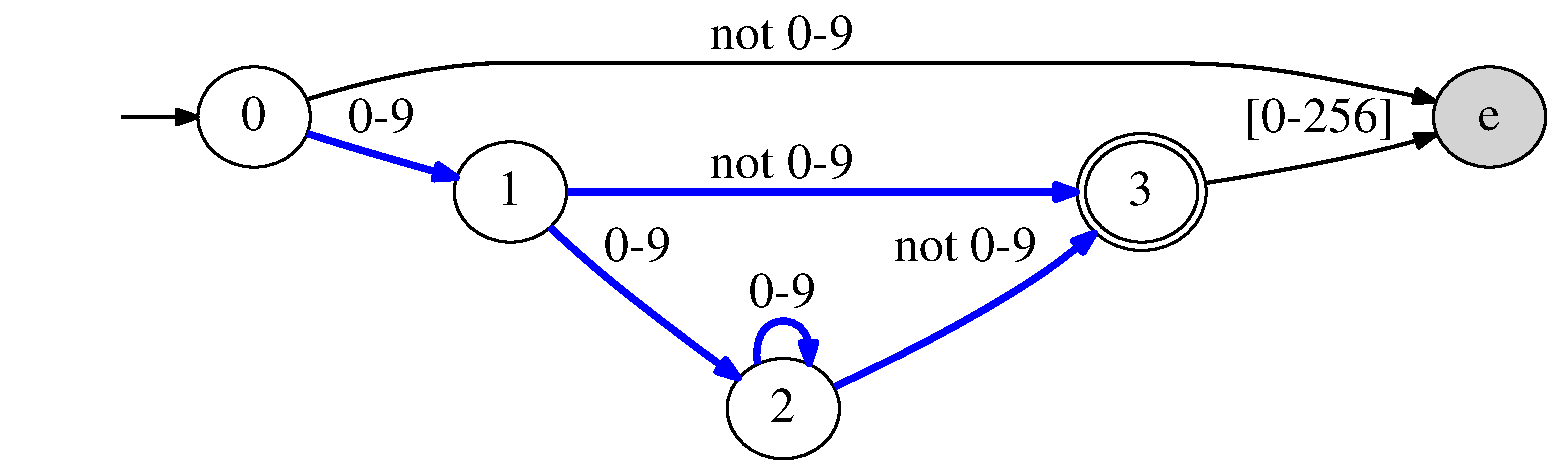
\includegraphics[width=0.45\textwidth]{figures/digits}
	\vspace{-12pt}
	\caption{Full-match DFA from RE2~\cite{re2} for the regular expression {\tt \textbackslash d+}. 
	RE2  interprets every string as a byte stream; the range of bytes is {\tt [0-256]} where {\tt [256]} is added to mark the end of a string. Thus, the input string ``2'' would be represented as {\tt [50 256]} and traverse the following path: $0 \rightarrow 1 \rightarrow 3$. 
	The edges marked \emph{0-9} represent the byte range {\tt [48-57]}; edges \emph{not 0-9} represent the byte ranges {\tt [0-47][58-256]}. }
	%State 2 is the initial state. State 5 is a final matching state. State 1 is a final non-matching state. 
	%\todo{I thought we discussed that non-matching states will all have a single circle, not a double-circle, as the double-circle indicates matching. Please fix. State 1 is a non-matching state with no outgoing edges. This is OK. We don't need to mark it as special.}
%	\todo{is this a first-match DFA?}
%    0-9 are the characters accepted in state transitions. It can also be written as [48-57]. The numbers in square brackets are accepted bytes in decimal in state transitions. [256] indicates there are no more bytes from the input string. The arrows colored blue represent transitions in successful matches.}
	\label{fig:static}    
	\vspace{-12pt}
\end{figure}

%Similar to the DFA in Figure~\ref{fig:bug}, which was used for illustrating our motivation, the DFA in Figure~\ref{fig:static} is a fully specified DFA generated by the RE2 tool~\cite{re2}.
% which interprets every string as a byte stream; the range of bytes is [0-256] where [256] is added to mark the end of a string. Thus, the input string ``2'' would be represented as [50 256] and traverse the following path: $0 \rightarrow 1 \rightarrow 3$. 
%	The edges marked \emph{0-9} represent the byte range [48-57]; edges \emph{not 0-9} represent the byte ranges [0-47][58-256]. 

At this point, we note that this is not the smallest DFA for the regular expression \verb!\d+!.  
%In our work, we build off the RE2~\cite{re2} tool, which generates the DFA shown in Figure~\ref{fig:match1}. 
As the same tool is used for the construction of all the  DFAs, any impact of the DFAs not being minimal  (e.g., extra nodes or edges compared to the minimal representation) is distributed throughout the whole data set and consistent across all experiments. 
%\adh{Does it matter whether the DFAs are minimal (except for performance)?}
While we refer to RE2~\cite{re2} for full details of the DFA construction, though some intuition is provided in Section~\ref{dfamapping}. 



	
%\textbf{Definition of Coverages.} The \emph{node coverage} is the percentage of visited nodes in the static DFA; the \emph{edge coverage} is the percentage of visited edges in the static DFA; the \emph{edge-pair coverage} is the proportion of visited edge pairs in the static DFA; the \emph{exit coverage} is the percentage of visited exits in the static DFA.
\subsection{Coverage Criteria} 
\label{coveragemetrics}
Given a set of strings $S$ and a DFA $G$, for all $n \in N$, we mark $n$ as \emph{covered} if $n$ is visited during the processing of some $s \in S$. Similarly, edges $e \in E$ and edge-pairs $ep \in EP$ are marked as \emph{covered} if they are traversed during the processing of some $s \in S$. The sets of covered nodes, edges, and edge-pairs are denoted $N_{cov}$, $E_{cov}$, and $EP_{cov}$, respectively. 
These sets are aggregated over all $s \in S$. 

As defined in prior work~\cite{ammann2016introduction}, we adopt coverage definitions for node coverage ($NC$), edge coverage ($EC$), and edge-pair coverage ($EPC$) as follows:  

%\footnote{The static DFA is the DFA generated with only the regular expression while the dynamic DFAs are the DFAs generated on-the-fly with the regular expression and its input strings. More details can be found in ~\ref{subsec:cov}}.
%Then the \emph{node coverage} is the percentage of reachable nodes in $G$; the \emph{edge coverage} is the percentage of reachable edges in the $G$; the \emph{edge-pair coverage} is the proportion of reachable edge pairs in $G$. We will omit the edge-pair coverage if there is only one edge in $G$.%; the \emph{exit coverage} is the percentage of reachable exits in $G$.

\begin{definition}[Node Coverage \%]
$NC = \displaystyle{100 \times \frac{\mid N_{cov} \mid}{ \mid N \mid}}$
\end{definition}

\begin{definition}[Edge Coverage \%]
$EC = \displaystyle{100 \times \frac{\mid E_{cov} \mid}{\mid E \mid}}$
\end{definition}

\begin{definition}[Edge-Pair Coverage \%]
$EPC = \displaystyle{100 \times \frac{\mid EP_{cov} \mid}{\mid EP \mid}}$
\end{definition}



%The regular expression `\textbackslash d+'  matches strings consisting only digits. From Figure~\ref{fig:static} we can see that its DFA graph contains five nodes (i.e., 0, 1, 2, 3, and E), seven edges (i.e., $\overrightarrow{0E}$,  $\overrightarrow{01}$,  $\overrightarrow{12}$,  $\overrightarrow{13}$,  $\overrightarrow{22}$,  $\overrightarrow{23}$, and  $\overrightarrow{3E}$), eight edge pairs (i.e., $\overrightarrow{012}$, $\overrightarrow{013}$, $\overrightarrow{122}$, $\overrightarrow{123}$, $\overrightarrow{13E}$, $\overrightarrow{222}$, $\overrightarrow{223}$, and $\overrightarrow{23E}$), one final matching node indicating a match (i.e., 3), and one final non-matching node, representing a non-match (i.e., E).
%\todo{for edge notation, using this notation is more standard. For paths of length 2, I'm not sure if we should use [1, 2, 3] as the book does, or  $\overrightarrow{123}$ for consistency. I'm leaning toward the latter, but for longer paths, we could use the former}.
%2~$\rightarrow$~2, 2~$\rightarrow$~1, 2~$\rightarrow$~3, 3~$\rightarrow$~4, 3~$\rightarrow$~5, 4~$\rightarrow$~4, 4~$\rightarrow$~5, and 5~$\rightarrow$~1), 


%2~$\rightarrow$~2~$\rightarrow$~1, 2~$\rightarrow$~2~$\rightarrow$~2, 2~$\rightarrow$~2~$\rightarrow$~3, 2~$\rightarrow$~3~$\rightarrow$~4, 2~$\rightarrow$~3~$\rightarrow$~5, 3~$\rightarrow$~4~$\rightarrow$~4, 3~$\rightarrow$~4~$\rightarrow$~5, 3~$\rightarrow$~5~$\rightarrow$~1, 4~$\rightarrow$~4~$\rightarrow$~4, 4~$\rightarrow$~4~$\rightarrow$~5, and 4~$\rightarrow$~5~$\rightarrow$~1), one final matching node indicating a match (i.e., 5), and one final non-matching node, representing a non-match (i.e., 1).


To illustrate the coverage levels, consider the graph $G$ for the regular expression \verb!\d+! in Figure~\ref{fig:static} and the string $s_0 = $``2'' with $S~=~\{s_0\}$. 
%Guided by Figure ~\ref{fig:static}, we can describe the process of matching a character `2' to the regular expression `\textbackslash d+'. 
Traversing $G$ visits $0 \rightarrow 1 \rightarrow 3$ (recall that ``2'' is interpreted as the byte stream [50 256]). Node~$3$ is the accept node, which denotes that the regular expression matches the input string (i.e., $s \in L(R)$). 
During the traversal of $G$, nodes \{0, 1, 3\} are visited, meaning that $N_{cov} = \{0, 1, 3\}$, $E_{cov} = \{\overrightarrow{01}, \overrightarrow{13}\}$, and $EP_{cov} = \{\overrightarrow{013}\}$. 
%Therefore, this process covers three visited nodes (i.e., 0, 1, and 3), two visited edges (i.e., $\overrightarrow{01}$, and $\overrightarrow{13}$), and one visited edge pair (i.e., $\overrightarrow{013}$). %This is a successful match. 
The coverage levels for \verb!\d+! by input strings $S = \{s_0\}$ are: $NC$ = 60\%(3/5), $EC$ =  28.6\% (2/7), and $EPC$ =  12.5\% (1/8).% 4) EXC 0\%(0/2).
%2~$\rightarrow$~1, 2~$\rightarrow$~3, and 3~$\rightarrow$~5
%2~$\rightarrow$~3~$\rightarrow$~5



%\todo{check consistency of state vs node}

Next, consider adding the string $s_1$ =``1001'', which is interpreted as the byte stream {\tt [49 48 48 49 256]}. Now, $S = \{s_0, s_1\}$.
Traversing $G$ on $s_1$ traverses the following path: $0 \rightarrow 1 \rightarrow 2 \rightarrow 2 \rightarrow 2 \rightarrow 3$, adding node~$2$ to $N_{cov}$, edges  $\overrightarrow{12}$, $\overrightarrow{22}$, and $\overrightarrow{23}$ to $E_{cov}$, and edge-pairs $\overrightarrow{012}$, $\overrightarrow{122}$, $\overrightarrow{222}$, and $\overrightarrow{223}$ to $EP_{cov}$. 
%Matching the regular expression `\textbackslash d+' with the input `1001' leads to a different process. The DFA transitions from state 2 to state 3 with the byte `1', from state 3 to state 4 with the byte `0', stays in state 4 with the bytes `0' and `1', and from state 4 to matching end state 5 with end indicator byte 256. This DFA graph covers four visited nodes (i.e., 0, 1, 2, and 3), four visited edges (i.e., $\overrightarrow{01}$, $\overrightarrow{12}$, $\overrightarrow{22}$, and $\overrightarrow{23}$), and four visited edge pairs (i.e., $\overrightarrow{012}$, $\overrightarrow{122}$, $\overrightarrow{222}$, and $\overrightarrow{223}$). The edge pair $\overrightarrow{123}$ looks feasible, but it is not visited in this specific process. 
As a result, the coverage levels for the regular expression \verb!\d+! by input strings $S = \{s_0, s_1\}$ are: 
$NC$ = 80\% (4/5), $EC$ = 71.4\% (5/7), and $EP$ = 62.5\% (5/8).
%2~$\rightarrow$~1, 2~$\rightarrow$~3, 3~$\rightarrow$~4, 4~$\rightarrow$~4, and 4~$\rightarrow$~5
%2~$\rightarrow$~3~$\rightarrow$~4, 3~$\rightarrow$~4~$\rightarrow$~4, 3~$\rightarrow$~4~$\rightarrow$~5, 4~$\rightarrow$~4~$\rightarrow$~4, and 4~$\rightarrow$~4~$\rightarrow$~5

As an example of a non-matching string, let $s_2$ = ``u'', which is interpreted as the byte stream {\tt [117 256]}. 
The path traversed in $G$ is $0 \rightarrow e$; after reaching $e$, the processing stops. 
Node $e$ is added to $N_{cov}$, edge $\overrightarrow{0e}$ is added to $E_{cov}$, and there is no change to $EP_{cov}$. 
Considering $S = \{s_0, s_1, s_2\}$, the combined coverage levels are: $NC$ = 100\% (5/5), $EC$ = 85.7\% (6/7), and $EPC$ =  62.5\% (5/8). %4) EXC 50\%(1/2).
%, and one exit (i.e., $\overrightarrow{21}$)
%2~$\rightarrow$~2 and 2~$\rightarrow$~1
%2~$\rightarrow$~2~$\rightarrow$~2, 2~$\rightarrow$~2~$\rightarrow$~1
%2~$\rightarrow$~1
%Because `u' does not belong to the range [48-57], the DFA transitions directly from the start state 2 to the final non-matching state 1. It covers only two nodes (i.e., 1 and 2), one edge (i.e., 2~$\rightarrow$~1), and one exit (i.e., 2~$\rightarrow$~1). The test coverages of the regular expression `\textbackslash d+' by input string `u' are: 1) NC 40\%(2/5); 2) EC 12.5\%(1/8); 3) EPC 0\%(0/11); 4) EXC 50\%(1/2).

For another example of a non-matching string, let $s_3$ = ``100u'', which is interpreted as the byte stream {\tt [49 48 48 117 256]}. 
The path traversed in $G$ is $0 \rightarrow 1 \rightarrow 2 \rightarrow 2 \rightarrow3 \rightarrow e$.
While this input visits all nodes in $G$, $NC = 100\%$ already, so no nodes are added to $N_{cov}$.
 Edge $\overrightarrow{3e}$ is added to $E_{cov}$, edge-pair $\overrightarrow{23e}$ is added to $EP_{cov}$. 
Considering $S = \{s_0, s_1, s_2, s_3\}$, the combined coverage levels are: $NC$ = 100\% (5/5), $EC$ = 100\% (7/7), and $EPC$ =  75\% (6/8). 


For each coverage metric, we compute coverage over the entire set of input strings, \emph{total}, and two subsets: \emph{success}, and \emph{failure}. 
The numbers reported in this section are for the \emph{total} set of input strings, that is, $S = \{s_0, s_1, s_2, s_3\}$. 
After, we split the input strings into those that terminate in an accept state in $N_m$, which we call $S_{succ}$, and those that  terminate in the error state $N_e$, which we call $S_{fail}$. With this example, $S_{succ} = \{s_0, s_1\}$ and $S_{fail} = \{s_2, s_3\}$.

Table~\ref{coverageExample} presents a summary of the coverage levels for each set of input strings. 
%To achieve high EC and EPC, we need to combine both successful matchings $S_{succ}$ and failed matchings $S_{fail}$.
Achieving 100\% for any of the coverage metrics is infeasible for $S_{succ}$ alone because the error state $e$ will never be reached, missing that node and the edges leading to it. 
In this example,  EC for $S_{succ}$ is 71.4\% while EC for $S$ is 100\%.

%The edge-pair coverage for all input strings is only 75\%. To get 100\% coverage of EPC, more inputs are needed. For example, adding string `10' will cover $\overrightarrow{123}$ and adding string `1u' will cover $\overrightarrow{13e}$. 
Achieving 100\% coverage for $EPC$ is the most difficult, but it is possible in this example. 
 The missing edge-pairs are computed by $EP \setminus EP_{cov} = \{\overrightarrow{123}, \overrightarrow{13e}\}$. Two additional input strings can lead to 100\% EPC. Input ``1u'' would be interpreted as the byte stream {\tt [49 117 256]} and traverses the path $0 \rightarrow 1 \rightarrow 3 \rightarrow e$, hence covering $\overrightarrow{13e}$. Input ``11u'' would lead to byte stream {\tt [49 49 117 256]}, traverse the path  $0 \rightarrow 1 \rightarrow 2 \rightarrow  3 \rightarrow e$ and cover $\overrightarrow{123}$. 
%\todo{under what conditions is  impossible to achieve 100\% EPC?}

\begin{table}[tb]
\caption{Coverage of {\tt \textbackslash d+}:  $S = \{``2", ``1001", ``u", ``100u"\}$, \\$S_{succ} = \{``2", ``1001"\}$, and $S_{fail} = \{``u", ``100u"\}$.}
\label{coverageExample}
\vspace{-6pt}
\begin{tabular}{l | r r r}
		& $S$ 	& $S_{succ}$ 	& $S_{fail}$ \\ \hline
$NC$	& 100.0\%	& 80.0\%	 &	100.0\%	\\
$EC$	& 100.0\% & 71.4\% &	85.7\%	\\
$EPC$	& 75.0\%	& 62.5\% &	50.0\%	\\
\hline
\end{tabular}
\vspace{-12pt}
\end{table}

Note that it is possible to have a DFA which is simply two nodes connected by a single edge. Thus, edge pairs may not exist.  For this case, we treat edge-pair coverage as identical to edge coverage. Among the 15,096 regular expressions studied in this work, only two regular expressions have this structure. 

%During regular expression processing, given a string and a regular expression to match against, RE2 uses dynamically-generated DFAs, which are subsets of the static DFA. We compute coverage on this fully static DFA, We refer to RE2 documentation for full details of the construction, 
 

%Another failed matching example is shown by matching the input string `100u' to the regular expression `\textbackslash d+'. The DFA transitions from the initial node 0 to node 2 `100'. Node 2 then transitions to the accept node 3 with the character `u'. In this example, node 3 is not the final node because it continues transitioning to the final error node E with the input end indicator byte 256. Compared to the example of `1001', this process covers one more node (i.e., E), one more edge (i.e., $\overrightarrow{3E}$), same number of edge pairs (i.e., adds $\overrightarrow{23E}$ and misses $\overrightarrow{222}$). The test coverages of the regular expression `\textbackslash d+' by input string `100u' are: 1) NC 100\%(5/5); 2) EC 71.43\%(5/7); 3) EPC 50\%(4/8).
%%5~$\rightarrow$~1
%%4~$\rightarrow$~5~$\rightarrow$~1
%
%The accumulated coverages by input `2' and `1001' are: 1) NC 80\%(4/5); 2) EC 71.43\%(5/7); 3) EPC 62.5\%(5/8). %; 4) EXC 0\%(0/2).
%The accumulated coverages by input `u' and `100u' are: 1) NC 100\%(5/5); 2) EC 85.71\%(6/7); 3) EPC 50\%(4/8). %; 4) EXC 100\%(2/2). 
%If `2', `1001', `u', and `100u' consists of all tested input strings, then the overall test coverages of the regular expression `\textbackslash d+' are: 1) NC 100\%(5/5); 2) EC 100\%(7/7); 3) EP 75\%(6/8). To achieve a 100\% coverage of EPC, more inputs are needed. For example, adding string `10' will cover $\overrightarrow{123}$ and adding string `1u' will cover $\overrightarrow{13E}$.%; 4) EXC 100\%(2/2).
